\documentclass[12pt,a4paper]{article}

% Essential packages
\usepackage[utf8]{inputenc}
\usepackage[T1]{fontenc}
\usepackage[english]{babel}
\usepackage{amsmath,amsfonts,amssymb}
\usepackage{graphicx}
\usepackage{float}
\usepackage{subcaption}
\usepackage{booktabs}
\usepackage{listings}
\usepackage{xcolor}
\usepackage{hyperref}
\usepackage{algorithm}
\usepackage{algpseudocode}

% Enhanced formatting packages
\usepackage{tocloft}           % Better Table of Contents formatting
\usepackage{titlesec}          % Custom section formatting with colors
\usepackage{enumitem}          % Better list formatting and spacing
\usepackage{microtype}         % Micro-typography improvements for cleaner text
\usepackage{setspace}          % Line spacing control
\usepackage{colortbl}          % Color in tables for better visual appeal
\usepackage{fancyhdr}          % Custom headers and footers
\usepackage{url}               % Better URL formatting
\usepackage{caption}           % Enhanced caption formatting
\usepackage{placeins}          % Better float placement control

% Geometry with improved margins
\usepackage[margin=2.5cm]{geometry}

% Page style setup
\pagestyle{fancy}
\fancyhf{}                     % Clear all header/footer fields
\rhead{Image Segmentation using Graph-Based Methods}
\lhead{Digital Image Processing}
\rfoot{Page \thepage}

% Paragraph formatting for better readability
\setlength{\parindent}{0pt}    % No paragraph indentation (modern style)
\setlength{\parskip}{8pt}      % Add space between paragraphs instead

% Custom color scheme
\definecolor{sectcolor}{RGB}{70,30,80}        % Deep purple for sections
\definecolor{linkcolor}{RGB}{0,120,215}       % Professional blue for links
\definecolor{tableheader}{RGB}{240,240,255}   % Light blue for table headers
\definecolor{codebackground}{RGB}{248,248,248} % Light gray for code blocks

% Enhanced section formatting with colors
\titleformat{\section}
  {\normalfont\Large\bfseries\color{sectcolor}}{\thesection}{1em}{}
\titleformat{\subsection}
  {\normalfont\large\bfseries\color{sectcolor}}{\thesubsection}{1em}{}
\titleformat{\subsubsection}
  {\normalfont\normalsize\bfseries\color{sectcolor}}{\thesubsubsection}{1em}{}

% Hyperref setup for professional links
\hypersetup{
    colorlinks=true,
    linkcolor=linkcolor,        % Internal links (sections, figures, etc.)
    urlcolor=linkcolor,         % External URLs
    citecolor=linkcolor,        % Citations
    pdfborder={0 0 0},         % Remove boxes around links
    pdftitle={Image Segmentation using Graph-Based Methods},
    pdfauthor={Student Name},
    pdfsubject={Digital Image Processing}
}

% Enhanced list formatting
\setlist{itemsep=4pt, topsep=6pt, parsep=2pt}

% Improved code listing style
\lstset{
    language=Python,
    basicstyle=\footnotesize\ttfamily,
    keywordstyle=\color{blue}\bfseries,
    commentstyle=\color{green!60!black},
    stringstyle=\color{red},
    showstringspaces=false,
    breaklines=true,
    frame=single,
    numbers=left,
    numberstyle=\tiny\color{gray},
    backgroundcolor=\color{codebackground},  % Light background for code
    captionpos=b,                            % Caption below code
    tabsize=4,                               % Tab size
    showstringspaces=false,                  % Don't show spaces in strings
    breakatwhitespace=true                   % Break lines at whitespace
}

% Enhanced algorithm formatting
\renewcommand{\algorithmicrequire}{\textbf{Input:}}
\renewcommand{\algorithmicensure}{\textbf{Output:}}

% Better caption formatting
\captionsetup{
    labelfont=bf,              % Bold labels (Figure 1:, Table 1:, etc.)
    textfont=it,               % Italic caption text
    labelsep=colon,            % Colon after label
    margin=10pt                % Margin around captions
}

% Title page information
\title{\Large \textbf{Image Segmentation using Graph-Based Methods: \\ Spectral Clustering and Normalized Cuts}}
\author{Fraidakis Ioannis\\
\small Department of Electrical and Computer Engineering\\
\small Aristotle University of Thessaloniki}
\date{June 2025}



\begin{document}

\maketitle
% \thispagestyle{empty}


\begin{abstract}
This report details the implementation and evaluation of graph-based image segmentation techniques, specifically focusing on spectral clustering and normalized cuts (N-Cuts). The project involves converting images into graph representations, implementing clustering algorithms, and demonstrating their performance on various datasets. The core components include an image-to-graph conversion module, a spectral clustering algorithm, and both non-recursive and recursive N-Cuts algorithms. Five demonstration scripts showcase the functionality, from testing on pre-built affinity matrices to full image segmentation pipelines and comparative analyses of different methods and parameter settings. The results highlight the strengths and weaknesses of each approach, the impact of parameter choices (like the number of clusters $k$, or N-Cuts thresholds $T_1, T_2$), and the differences between standard spectral clustering and the more balanced partitioning achieved by N-Cuts.
\end{abstract}


% \newpage

\section{Introduction}

Image segmentation is a fundamental problem in computer vision that involves partitioning an image into meaningful regions, often referred to as superpixels. Traditional pixel-based approaches often fail to capture the global structure and relationships within images. Graph-based segmentation methods address this limitation by modeling the image as a weighted graph, where pixels are nodes and edge weights encode similarity relationships.

This project implements and explores three key aspects of graph-based image segmentation:
\begin{enumerate}
    \item \textbf{Image-to-Graph Conversion}: Transforming raw image data into an affinity matrix that represents a fully-connected graph of pixels.
    \item \textbf{Spectral Clustering}: A technique that uses the eigenvalues (spectrum) of the graph Laplacian matrix to perform dimensionality reduction before clustering in a lower-dimensional space.
    \item \textbf{Normalized Cuts (N-Cuts)}: An advanced graph partitioning method that aims to find balanced clusters by minimizing a normalized cut criterion, often leading to more perceptually meaningful segmentations. This includes non-recursive, recursive, and binary N-Cuts implementations.
\end{enumerate}

The theoretical foundation builds upon spectral graph theory, where the eigenstructure of matrices derived from graphs reveals important clustering information. The smallest (nonzero) eigenvalues of the Laplacian matrix correspond to the most natural cuts in the graph, making them ideal for segmentation tasks.


Through a series of demonstrations, we will analyze the behavior of these algorithms, compare their outputs, and discuss their suitability for various image segmentation tasks. The provided dataset includes a pre-built affinity matrix (\texttt{d1a}) and two RGB images (\texttt{d2a}, \texttt{d2b}) for testing.






\section{Theoretical Background}

Graph-based image segmentation provides a powerful paradigm shift from traditional pixel-level analysis to a graph-theoretic framework. This approach models an image as a weighted graph, where pixels are represented as vertices and the relationships between them as weighted edges. Such a representation allows the application of sophisticated spectral analysis techniques to achieve robust image segmentation.

\subsection{Graph Representation of Images}
\label{subsec:graph_representation}

The cornerstone of graph-based segmentation is the transformation of an image into a weighted graph $G = (V, E)$. In this graph, the set of vertices $V$ corresponds to the image pixels, and the set of edges $E$ represents the relationships between these pixels, quantified by weights. For an $M \times N$ image, each pixel $(i,j)$ becomes a node, resulting in $n = M \cdot N$ vertices in the graph.

The affinity, or weight $W_{uv} \in \mathbb{R}^{n \times n}$, between any two pixels $u$ and $v$ quantifies their similarity, typically based on features like color or intensity. A common method to define this affinity is through an exponential weighting function:
\begin{equation}
W_{uv} = \exp(-d(I_u, I_v))
\end{equation}
where $d(I_u, I_v)$ is the Euclidean distance between the feature vectors (e.g., color values in a C-channel image) of pixels $u$ and $v$:
\begin{equation}
d(I_u, I_v) = \sqrt{\sum_{c=1}^{C} (I_u^{(c)} - I_v^{(c)})^2}
\end{equation}
This formulation ensures that pixels with high similarity (small Euclidean distance) have a high affinity ($W_{uv} \rightarrow 1$), whereas dissimilar pixels ($d \rightarrow \infty$) have a low affinity ($W_{uv} \rightarrow 0$). The resulting graph is fully connected, although many edge weights may be negligible.

\subsection{Spectral Clustering Theory}
\label{subsec:spectral_theory}

Spectral clustering leverages the eigenstructure (spectrum) of matrices derived from the graph, most notably the graph Laplacian, to perform dimensionality reduction. This process projects the data (pixels) into a lower-dimensional space where cluster structures are more apparent, facilitating segmentation by traditional clustering algorithms like K-means.

The general procedure for spectral clustering is outlined below:
\begin{algorithm}[H]
\caption{Spectral Clustering Algorithm}
\begin{algorithmic}[1]
\State Construct the affinity matrix $W$ from the input data 
\State Compute the degree matrix $D$, a diagonal matrix where $D_{ii} = \sum_{j=1}^{n} W_{ij}$.
\State Compute the unnormalized graph Laplacian matrix $L = D - W$.
\State Determine the $k$ smallest eigenvalues of $L$ and their corresponding eigenvectors.
\State Form a matrix $U \in \mathbb{R}^{n \times k}$ using these $k$ eigenvectors as its columns, sorted by their associated eigenvalues ($U = [v_1 | v_2 | \ldots | v_k])$.
\State Apply K-means clustering to partition these $n$ points into $k$ distinct clusters.
\State Assign the cluster labels obtained from K-means to the original data points (pixels).
\end{algorithmic}
\end{algorithm}

\subsubsection*{Mathematical Foundation}
The theoretical underpinning of spectral clustering lies in the properties of the graph Laplacian matrix $L = D - W$. The eigenvectors of $L$ associated with its smallest eigenvalues reveal the underlying connectivity and partitioning of the graph. Specifically, for the eigenvalue problem $Lx = \lambda x$, the eigenvector corresponding to the second smallest eigenvalue (known as the Fiedler vector, with the Fiedler value $\lambda_2$) provides an optimal (in a relaxed sense) binary partition of the graph.

\subsection{Normalized Cuts Theory}
\label{subsec:ncuts_theory}

The Normalized Cuts (N-Cuts) criterion was developed to address limitations in standard spectral clustering approaches. While spectral clustering using the unnormalized Laplacian can effectively identify cluster structures, it sometimes produces unbalanced partitions where small, loosely connected components get isolated from the main clusters. N-Cuts introduces a normalization term that considers the "volume" or total connection strength of each partition, leading to more balanced and perceptually meaningful segmentations.


\subsubsection{Mathematical Formulation}

For a binary partition $(A, B)$ where $A \cup B = V$ and $A \cap B = \emptyset$, the normalized cut criterion is:

\begin{equation}
\text{Ncut}(A,B) = \frac{\text{cut}(A,B)}{\text{assoc}(A,V)} + \frac{\text{cut}(A,B)}{\text{assoc}(B,V)}
\end{equation}

where the key terms are defined as:
\begin{align}
\text{cut}(A,B) &= \sum_{u \in A, v \in B} W_{uv} \quad \text{(inter-partition connectivity)} \\
\text{assoc}(A,V) &= \sum_{u \in A, t \in V} W_{ut} \quad \text{(total connectivity of partition A)}
\end{align}

\textbf{Alternative Formulation}, often used in practice is:
\begin{equation}
\text{Ncut}(A,B) = 2 - \text{Nassoc}(A,B)
\end{equation}
where:
\begin{equation}
\text{Nassoc}(A,B) = \frac{\text{assoc}(A,A)}{\text{assoc}(A,V)} + \frac{\text{assoc}(B,B)}{\text{assoc}(B,V)}
\end{equation}

and $\text{assoc}(A,A) = \sum_{u \in A, v \in A} W_{uv}$ represents the internal connectivity within partition $A$.


\subsubsection{Non-Recursive N-Cuts Algorithm}

A key distinction of the N-Cuts algorithm from standard spectral clustering (using the unnormalized Laplacian) is its formulation as a \textbf{generalized eigenvalue problem}:
\begin{equation}
Lx = \lambda Dx
\end{equation}
Solving this system, typically for the eigenvectors corresponding to the smallest eigenvalues (excluding the trivial smallest one), provides the basis for partitioning. This formulation inherently incorporates the degree normalization, which is crucial for achieving balanced cuts and avoiding the bias toward isolating small, weakly connected components that can occur with unnormalized approaches.

\subsubsection{Recursive Partitioning Strategy}

The Recursive N-Cuts algorithm extends the standard N-Cuts approach by repeatedly applying binary (k=2 splits) N-Cuts to automatically determine an appropriate number of clusters. It operates by iteratively subdividing the graph (or subgraphs) in a data-driven manner, where each recursive step involves a binary split decision. The partitioning process for a given cluster ceases based on predefined criteria:

\begin{itemize}
    \item \textbf{Minimum Size Threshold ($T_1$)}: A partition is not split further if any of the resulting sub-partitions would contain fewer than $T_1$ vertices. This prevents over-segmentation into impractically small regions.
    \item \textbf{N-Cut Value Threshold ($T_2$)}: A split is rejected if its N-Cut value exceeds a threshold $T_2$. This ensures that only high-quality partitions (i.e., those with low N-Cut values, indicating good separation and balance) are accepted.
\end{itemize}
This adaptive strategy allows the segmentation to reflect the natural structure of the image data, rather than imposing a fixed number of clusters.





\section{Implementation Framework}

\subsection{Code Architecture}
The project is structured into a collection of Python modules, each dedicated to specific functionalities within the graph-based image segmentation pipeline. This modular design enhances code organization, reusability, and maintainability. The core modules are:

\begin{itemize}
    
    \item \textbf{\texttt{image\_to\_graph.py}}: Implements the \href{Code/image_to_graph.py}{\texttt{image\_to\_graph}} function, which converts an input image into an affinity matrix representing a fully-connected graph of pixels. It serves as the critical bridge between spatial image data and graph-theoretic analysis, detailed in Section~\ref{subsec:image_to_graph_impl}.
    
    \item \textbf{\texttt{spectral\_clustering.py}}: Contains the \href{Code/spectral_clustering.py}{\texttt{spectral\_clustering}} function, which performs segmentation using the eigenvalues of the graph Laplacian. It performs eigenvalue decomposition of the graph Laplacian and applies K-means clustering in the reduced eigenspace. The methodology leverages spectral graph theory for dimensionality reduction before clustering, as explained in Section~\ref{subsec:spectral_impl}.
    
    \item \textbf{\texttt{n\_cuts.py}}: Provides implementations for Normalized Cuts, including the \href{Code/n_cuts.py}{\texttt{n\_cuts}} function for k-way partitioning, \href{Code/n_cuts.py}{\texttt{calculate\_n\_cut\_value}} for evaluating binary splits, and \href{Code/n_cuts.py}{\texttt{n\_cuts\_recursive}} for adaptive segmentation  with automatic cluster number determination. The algorithmic details are discussed in Section~\ref{subsec:ncuts_impl}.
    
    \item \textbf{\texttt{demo\_utils.py}}: A utility module (\href{Code/demo_utils.py}{\texttt{demo\_utils.py}}) containing helper functions for visualization and analysis, used across various demonstrations.
    
    \item \textbf{\texttt{demo1.py} -- \texttt{demo3c.py}}: A series of scripts (\href{Code/demo1.py}{\texttt{demo1.py}}, \href{Code/demo2.py}{\texttt{demo2.py}}, \href{Code/demo3a.py}{\texttt{demo3a.py}}, \href{Code/demo3b.py}{\texttt{demo3b.py}}, \href{Code/demo3c.py}{\texttt{demo3c.py}}) that demonstrate and test the implemented algorithms with various configurations and datasets.
    
    \item \textbf{\texttt{run\_all.py}}: A script (\href{Code/run_all.py}{\texttt{run\_all.py}}) to execute all demonstration scripts sequentially and organize the output results into a \texttt{results/} directory.

\end{itemize}


\subsection{Technical Dependencies}
The project is implemented in Python and leverages several scientific computing libraries:
\begin{itemize}
    \item \textbf{NumPy}: Core library for numerical computations and array manipulations, providing the foundation for image representation, affinity matrix operations, and all algorithmic calculations involving large matrices.
    \item \textbf{SciPy}:
        \begin{itemize}
            \item \texttt{scipy.io.loadmat}: Used in \href{Code/demo_utils.py}{\texttt{demo\_utils.py}} (via \texttt{load\_demo\_images}) for loading MATLAB data files (\texttt{.mat})
            \item \texttt{scipy.sparse.linalg.eigsh}: For efficient eigenvalue computation on large symmetric matrices. It is used in \href{Code/spectral_clustering.py}{\texttt{spectral\_clustering.py}}, and \href{Code/n_cuts.py}{\texttt{n\_cuts.py}}. This is crucial for performance with affinity matrices derived from images.
        \end{itemize}
    \item \textbf{Scikit-learn}:
        \begin{itemize}
            \item \texttt{sklearn.cluster.KMeans}: For the K-means clustering step in both \href{Code/n_cuts.py}{\texttt{n\_cuts}} and \href{Code/spectral_clustering.py}{\texttt{spectral\_clustering}}. \texttt{random\_state=1} is used for reproducibility.
        \end{itemize}
    \item \textbf{Matplotlib}: Employed for comprehensive visualization of segmentation results, statistical analysis plots, and comparative result displays across all demonstration scripts (\texttt{demo*.py}).
\end{itemize}


\section{Proposed Algorithm Implementations}

This section details the specific algorithmic implementations of the theoretical concepts presented above, including optimization strategies and practical considerations for efficient computation.

\subsection{Image-to-Graph Conversion}
\label{subsec:image_to_graph_impl}

The \texttt{image\_to\_graph} function implements the transformation from pixel space to graph representation through efficient computation using SciPy's distance utilities.

\begin{algorithm}[H]
\caption{Image-to-Graph Conversion}
\begin{algorithmic}[1]
\Function{image\_to\_graph}{$img\_array$}
    \State Validate input array dimensions and type
    \State Extract dimensions: $M, N, C \gets img\_array.shape$
    \State $n\_pixels \gets M \times N$
    \State $pixels \gets$ reshape($img\_array$, $(n\_pixels, C)$) \Comment{Flatten to pixel array}
    \State $distances \gets$ pdist($pixels$, metric='euclidean') \Comment{Euclidean distance}
    \State $distances \gets$ squareform($distances$) \Comment{Convert to full matrix}
    \State $affinity\_mat \gets \exp(-distances)$
    \State \Return $affinity\_mat$
\EndFunction
\end{algorithmic}
\end{algorithm}

\textbf{Key Implementation Features:}
\begin{itemize}
    \item \textbf{Input Validation}: The function first ensures the input is a valid 3D NumPy array with dimensions $[M, N, C]$, corresponding to image height, width, and color channels.

    \item \textbf{Image Reshaping}: The input image of size $M \times N \times C$ is flattened into a 2D array of shape $(M \cdot N) \times C$. Each row in this new array represents a single pixel's feature vector (e.g., its RGB values).
    \item \textbf{Efficient Distance Computation}: Pairwise distances between all pixels are computed efficiently using \texttt{scipy.spatial.distance.pdist}, which avoids explicit Python loops and leverages optimized backend code.

    \item \textbf{Choice of Distance Metric}: The core of the affinity calculation relies on measuring the "distance" between pixel feature vectors. The implementation allows for different metrics, with Euclidean and Chebyshev being the most relevant:
    \begin{itemize}
        \item \textbf{Euclidean Distance (L$_2$ norm)}: Calculates the standard straight-line distance in the color space. It is a good general-purpose metric that holistically considers differences across all color channels.
        \begin{equation}
        d_{\text{Euclidean}}(I_u, I_v) = \sqrt{\sum_{c=1}^{C} (I_u^{(c)} - I_v^{(c)})^2}
        \end{equation}
        \item \textbf{Chebyshev Distance (L$_\infty$ norm)}: Measures the maximum difference along any single color channel. This metric is particularly effective for separating regions where the primary distinction lies in one dominant color component.
        \begin{equation}
        d_{\text{Chebyshev}}(I_u, I_v) = \max_{c=1}^{C} |I_u^{(c)} - I_v^{(c)}|
        \end{equation}
    \end{itemize}

    \item \textbf{Affinity Matrix Generation}: The resulting pairwise distance matrix is converted into an affinity (or similarity) matrix $W$ using a Gaussian kernel: $W_{ij} = \exp(-d_{ij})$. 
    \item \textbf{Graph Representation}: The output is a dense $n \times n$ affinity matrix, where $n = M \cdot N$. This matrix represents a fully-connected graph where every pixel is a node connected to every other pixel.
\end{itemize}

\textbf{Design Rationale:}
The choice between Euclidean and Chebyshev distance depends on the image content. Euclidean distance is robust and works well for images with smooth gradients or where overall color similarity defines the segments. In contrast, Chebyshev distance excels at identifying sharp boundaries defined by a significant shift in a single color channel, making it suitable for images with distinct, flat-colored regions.


\subsection{Spectral Clustering Implementation}
\label{subsec:spectral_impl}

The \texttt{spectral\_clustering} function implements the standard spectral clustering algorithm using the unnormalized graph Laplacian. It takes an affinity matrix and the desired number of clusters, $k$, as input and returns an array of cluster labels for each node (pixel).

\begin{algorithm}[H]
    \caption{Spectral Clustering Algorithm}
    \begin{algorithmic}[1]
        \Function{spectral\_clustering}{$W$, $k$}
            \State $D \gets \text{diag}(\sum_{j} W_{ij})$ \Comment{Compute the Degree Matrix}
            \State $L \gets D - W$ \Comment{Compute the Unnormalized Graph Laplacian}
            \State $\lambda, V \gets \text{eigsh}(L, k, \text{which='SM'})$ \Comment{Find $k$ smallest eigenvalues and eigenvectors}
            \State $labels \gets \text{KMeans}(V, k, \text{random\_state=1})$ \Comment{Cluster eigenvectors}
            \State \Return $labels$
        \EndFunction
    \end{algorithmic}
\end{algorithm}

The spectral clustering implementation proceeds in the following stages:

\begin{enumerate}
    \item \textbf{Degree Matrix Construction}: The degree matrix $D$ is computed as a diagonal matrix where each diagonal element $D_{ii}$ represents the sum of affinities for pixel $i$: $D_{ii} = \sum_{j=1}^{n} W_{ij}$. This quantifies the total connectivity of each pixel to all others.
    
    \item \textbf{Laplacian Matrix Formation}: The unnormalized graph Laplacian is constructed as $L = D - W$, where $W$ is the $affinity\_matrix$. 
    
    \item \textbf{Eigenvalue Decomposition}: The core of the spectral method involves computing the $k$ smallest eigenvalues and their corresponding eigenvectors for the Laplacian matrix $L$. For computational efficiency with large, symmetric matrices, this is performed using \texttt{scipy.sparse.linalg.eigsh} with the parameter \texttt{which='SM'} to specifically target the eigenvalues with the smallest magnitude. 
        
    \item \textbf{K-means Clustering}: The rows of matrix $V$ (which represent the nodes in the $k$-dimensional eigenspace) are clustered into $k$ groups using the K-means algorithm. \texttt{sklearn.cluster.KMeans} is used with \texttt{random\_state=1} for reproducibility.
\end{enumerate}

The implementation leverages sparse matrix operations when appropriate and uses the symmetric properties of the Laplacian matrix to improve computational efficiency. 

\subsection{N-Cuts Implementation}
\label{subsec:ncuts_impl}

The N-Cuts algorithm is implemented in {\texttt{n\_cuts.py}}. This includes a function for k-way partitioning ({\texttt{n\_cuts}}), a function to compute the N-Cut value for a binary partition ({\texttt{calculate\_n\_cut\_value}}), and a function for recursive N-Cuts ({\texttt{n\_cuts\_recursive}}).

\subsubsection{Core N-Cuts Algorithm}

The non-recursive {\texttt{n\_cuts} function performs k-way partitioning by solving a generalized eigenvalue problem.

\begin{algorithm}[H]
    \caption{N-Cuts K-way Partitioning}
    \begin{algorithmic}[1]
        \Function{n\_cuts}{$W$, $k$}
            \State $D \gets$ diag($\sum_{j} W_{ij}$) \Comment{Degree matrix}
            \State $L \gets D - W$ \Comment{Unnormalized Laplacian}
            \State $\lambda, V \gets \text{eigsh}(L, M=D, k, \text{which='SM'})$ \Comment{$Lv = \lambda Dv$}
            \State $labels \gets \text{KMeans}(V, k, \text{random\_state=1})$ \Comment{Cluster eigenvectors}
            \State \Return $cluster\_labels$
        \EndFunction
    \end{algorithmic}
\end{algorithm}

The N-Cuts algorithm differs from standard spectral clustering in the following aspects:

\begin{enumerate}
    \item \textbf{Generalized Eigenvalue Problem}: Instead of solving the standard eigenvalue problem $Lv = \lambda v$, it solves the \textbf{generalized eigenvalue problem} $Lv = \lambda Dv$. This is accomplished using \texttt{scipy.sparse.linalg.eigsh} with the degree matrix $D$ passed as the mass matrix argument ($M=D$).
        
    \item \textbf{Balanced Partitioning}: The degree normalization inherent in the generalized eigenvalue formulation encourages partitions that balance both cut cost and partition sizes, typically producing more perceptually meaningful segmentations.    
\end{enumerate}

\subsubsection{N-Cut Value Computation}
\label{subsec:ncuts_value_impl}

The {\texttt{calculate\_n\_cut\_value}} function computes the N-Cut value for a given binary partition of a graph, as defined by its affinity matrix and cluster labels.

\begin{algorithm}[H]
\caption{N-Cut Value Computation (Binary)}
\begin{algorithmic}[1]
    \Function{calculate\_n\_cut\_value}{$W, cluster\_idx$}
        \State $cluster\_A \gets \{i : cluster\_idx[i] = 0\}$
        \State $cluster\_B \gets \{i : cluster\_idx[i] = 1\}$
        
        \If{$|cluster\_A| = 0$ \textbf{or} $|cluster\_B| = 0$}
            \State \Return $2.0$ \Comment{Maximal n-cut value for degenerate case}
        \EndIf
        
        \State $degrees \gets \sum_{j} W_{ij}$ for all $i$ \Comment{Calculate node degrees}
        \State $assoc\_AV \gets \sum_{u \in cluster\_A} degrees[u]$ \Comment{Sum of degrees in cluster A}
        \State $assoc\_BV \gets \sum_{u \in cluster\_B} degrees[u]$ \Comment{Sum of degrees in cluster B}
        
        \If{$assoc\_AV < 10^{-10}$ \textbf{or} $assoc\_BV < 10^{-10}$}
            \State \Return $2.0$ \Comment{Handle zero associations}
        \EndIf
        
        \State $assoc\_AA \gets \sum_{u,v \in cluster\_A} W_{uv}$ \Comment{Internal connections in A}
        \State $assoc\_BB \gets \sum_{u,v \in cluster\_B} W_{uv}$ \Comment{Internal connections in B}
        
        \State $N\_assoc\_AB \gets \frac{assoc\_AA}{assoc\_AV} + \frac{assoc\_BB}{assoc\_BV}$
        \State $n\_cut\_value \gets 2.0 - N\_assoc\_AB$
        
        \State \Return $n\_cut\_value$
    \EndFunction
\end{algorithmic}
\end{algorithm}

The N-Cut value computation implements the theoretical formulation:

\begin{enumerate}
    \item \textbf{Partition Identification}: For each pair of clusters, the algorithm identifies the sets of vertices belonging to each partition.
    
    \item \textbf{Cut Calculation}: The cut value between partitions A and B is computed as the sum of edge weights crossing the partition boundary: $cut(A,B) = \sum_{u \in A, v \in B} W_{uv}$.
    
    \item \textbf{Association Calculation}: The total association of each partition with the entire graph is computed: $assoc(A,V) = \sum_{u \in A, v \in V} W_{uv}$.
    
    \item \textbf{Normalized Cut Formula}: The N-Cut value for the partition pair is calculated as: $Ncut(A,B) = \frac{cut(A,B)}{assoc(A,V)} + \frac{cut(A,B)}{assoc(B,V)}$.
    
    \item \textbf{Total N-Cut Summation}: For multi-way partitions, the total N-Cut value is the sum of pairwise N-Cut values across all partition pairs.
\end{enumerate}

This metric provides a quantitative measure of partition quality, where lower values indicate better cuts that minimize inter-cluster connectivity while maintaining balanced partition sizes.

\subsubsection{Recursive N-Cuts Implementation}
\label{subsec:ncuts_recursive_impl}

The \texttt{n\_cuts\_recursive} function implements adaptive segmentation that automatically determines the optimal number of clusters based on data-driven stopping criteria.


\begin{algorithm}[H]
\caption{Recursive N-Cuts}
\begin{algorithmic}[1]
\Function{n\_cuts\_recursive}{$affinity\_mat$, $T_1$, $T_2$}
    \State Initialize queue with entire graph: $\mathcal{Q} = \{(V, W)\}$
    \State Initialize final segments: $final\_segments = \emptyset$ 
    \While{queue not empty}
        \State $(subgraph, indices) \gets \text{dequeue}(\mathcal{Q})$
        \If{$|indices| < 2 \times T_1$} \Comment{Too small to split}
            \State  $final\_segments \leftarrow final\_segments \cup \{V_{\text{sub}}\}$
            \State \textbf{continue}
        \EndIf
        \State $binary\_labels \gets$ n\_cuts($subgraph$, $k=2$)
        \State Split indices into $A$ and $B$ based on $binary\_labels$
        \State $ncut\_value \gets$ calculate\_n\_cut\_value($subgraph$, $binary\_labels$)
        \If{$|A| < T_1$ \textbf{or} $|B| < T_1$ \textbf{or} $ncut\_value > T_2$} \Comment{Poor split quality}
            \State  $final\_segments \leftarrow final\_segments \cup \{V_{\text{sub}}\}$
        \Else
            \State Extract sub-affinity matrices for $A$ and $B$
            \State $\text{enqueue}(\mathcal{Q}, (A, W_A))$ and $\text{enqueue}(\mathcal{Q}, (B, W_B))$
        \EndIf
    \EndWhile
    \State \Return $final\_segments$
\EndFunction
\end{algorithmic}
\end{algorithm}

The recursive N-Cuts algorithm employs a sophisticated divide-and-conquer strategy:

\begin{enumerate}
    \item \textbf{Queue-Based Processing}: The algorithm maintains a queue of subgraphs to be processed, starting with the complete graph. This breadth-first approach ensures systematic exploration of the partition hierarchy.
    
    \item \textbf{Size-Based Stopping Criterion}: If a subgraph contains fewer than $2 \times T_1$ vertices, it cannot be meaningfully split into two clusters of minimum size $T_1$, so it becomes a final cluster.
    
    \item \textbf{Binary Split Evaluation}: Each sufficiently large subgraph undergoes binary N-Cuts partitioning. The algorithm computes the N-Cut value for this binary split to assess its quality.
    
    \item \textbf{Quality-Based Stopping Criteria}: A split is rejected if:
        \begin{itemize}
            \item Either resulting cluster would be smaller than $T_1$ vertices
            \item The N-Cut value exceeds the threshold $T_2$, indicating a poor-quality split
        \end{itemize}
    
    \item \textbf{Recursive Subdivision}: If the split passes quality tests, both resulting subgraphs are added to the processing queue for potential further subdivision. The corresponding sub-affinity matrices are extracted to maintain proper graph structure.
    
    \item \textbf{Adaptive Termination}: The process continues until no more beneficial splits can be found, automatically determining the optimal number of clusters based on the intrinsic structure of the data and the specified quality thresholds.
\end{enumerate}

The algorithm's key innovation lies in its adaptive nature—rather than requiring a predetermined number of clusters, it discovers the natural segmentation hierarchy present in the data. The parameters $T_1$ and $T_2$ provide user control over the granularity and quality of the final segmentation, making it particularly suitable for applications where the optimal number of segments is unknown a priori.









\section{Experimental Setup}

\subsection*{Test Dataset}

Our experiments utilized a carefully selected dataset consisting of three distinct components, each designed to evaluate different aspects of the graph-based segmentation algorithms:

\begin{itemize}
    \item \textbf{Pre-built Affinity Matrix (d1a)}: A $12 \times 12$ symmetric matrix representing a controlled graph structure. This matrix serves as a baseline for validating the spectral clustering implementation without the complexities introduced by image-to-graph conversion.
    
    \item \textbf{Test Image d2a}: A $50 \times 50$ RGB image featuring a simple three-stripe pattern with distinct colors (red, green, blue). This synthetic image provides an ideal test case with clear, well-defined boundaries and known ground truth segmentation.
    
    \item \textbf{Test Image d2b}: A $50 \times 50$ RGB image depicting a Mario character with complex spatial structure and multiple color regions. This image represents a more challenging segmentation scenario with natural object boundaries and varying textures.
\end{itemize}

\begin{figure}[H]
    \centering
    \begin{subfigure}{0.45\textwidth}
        \centering
        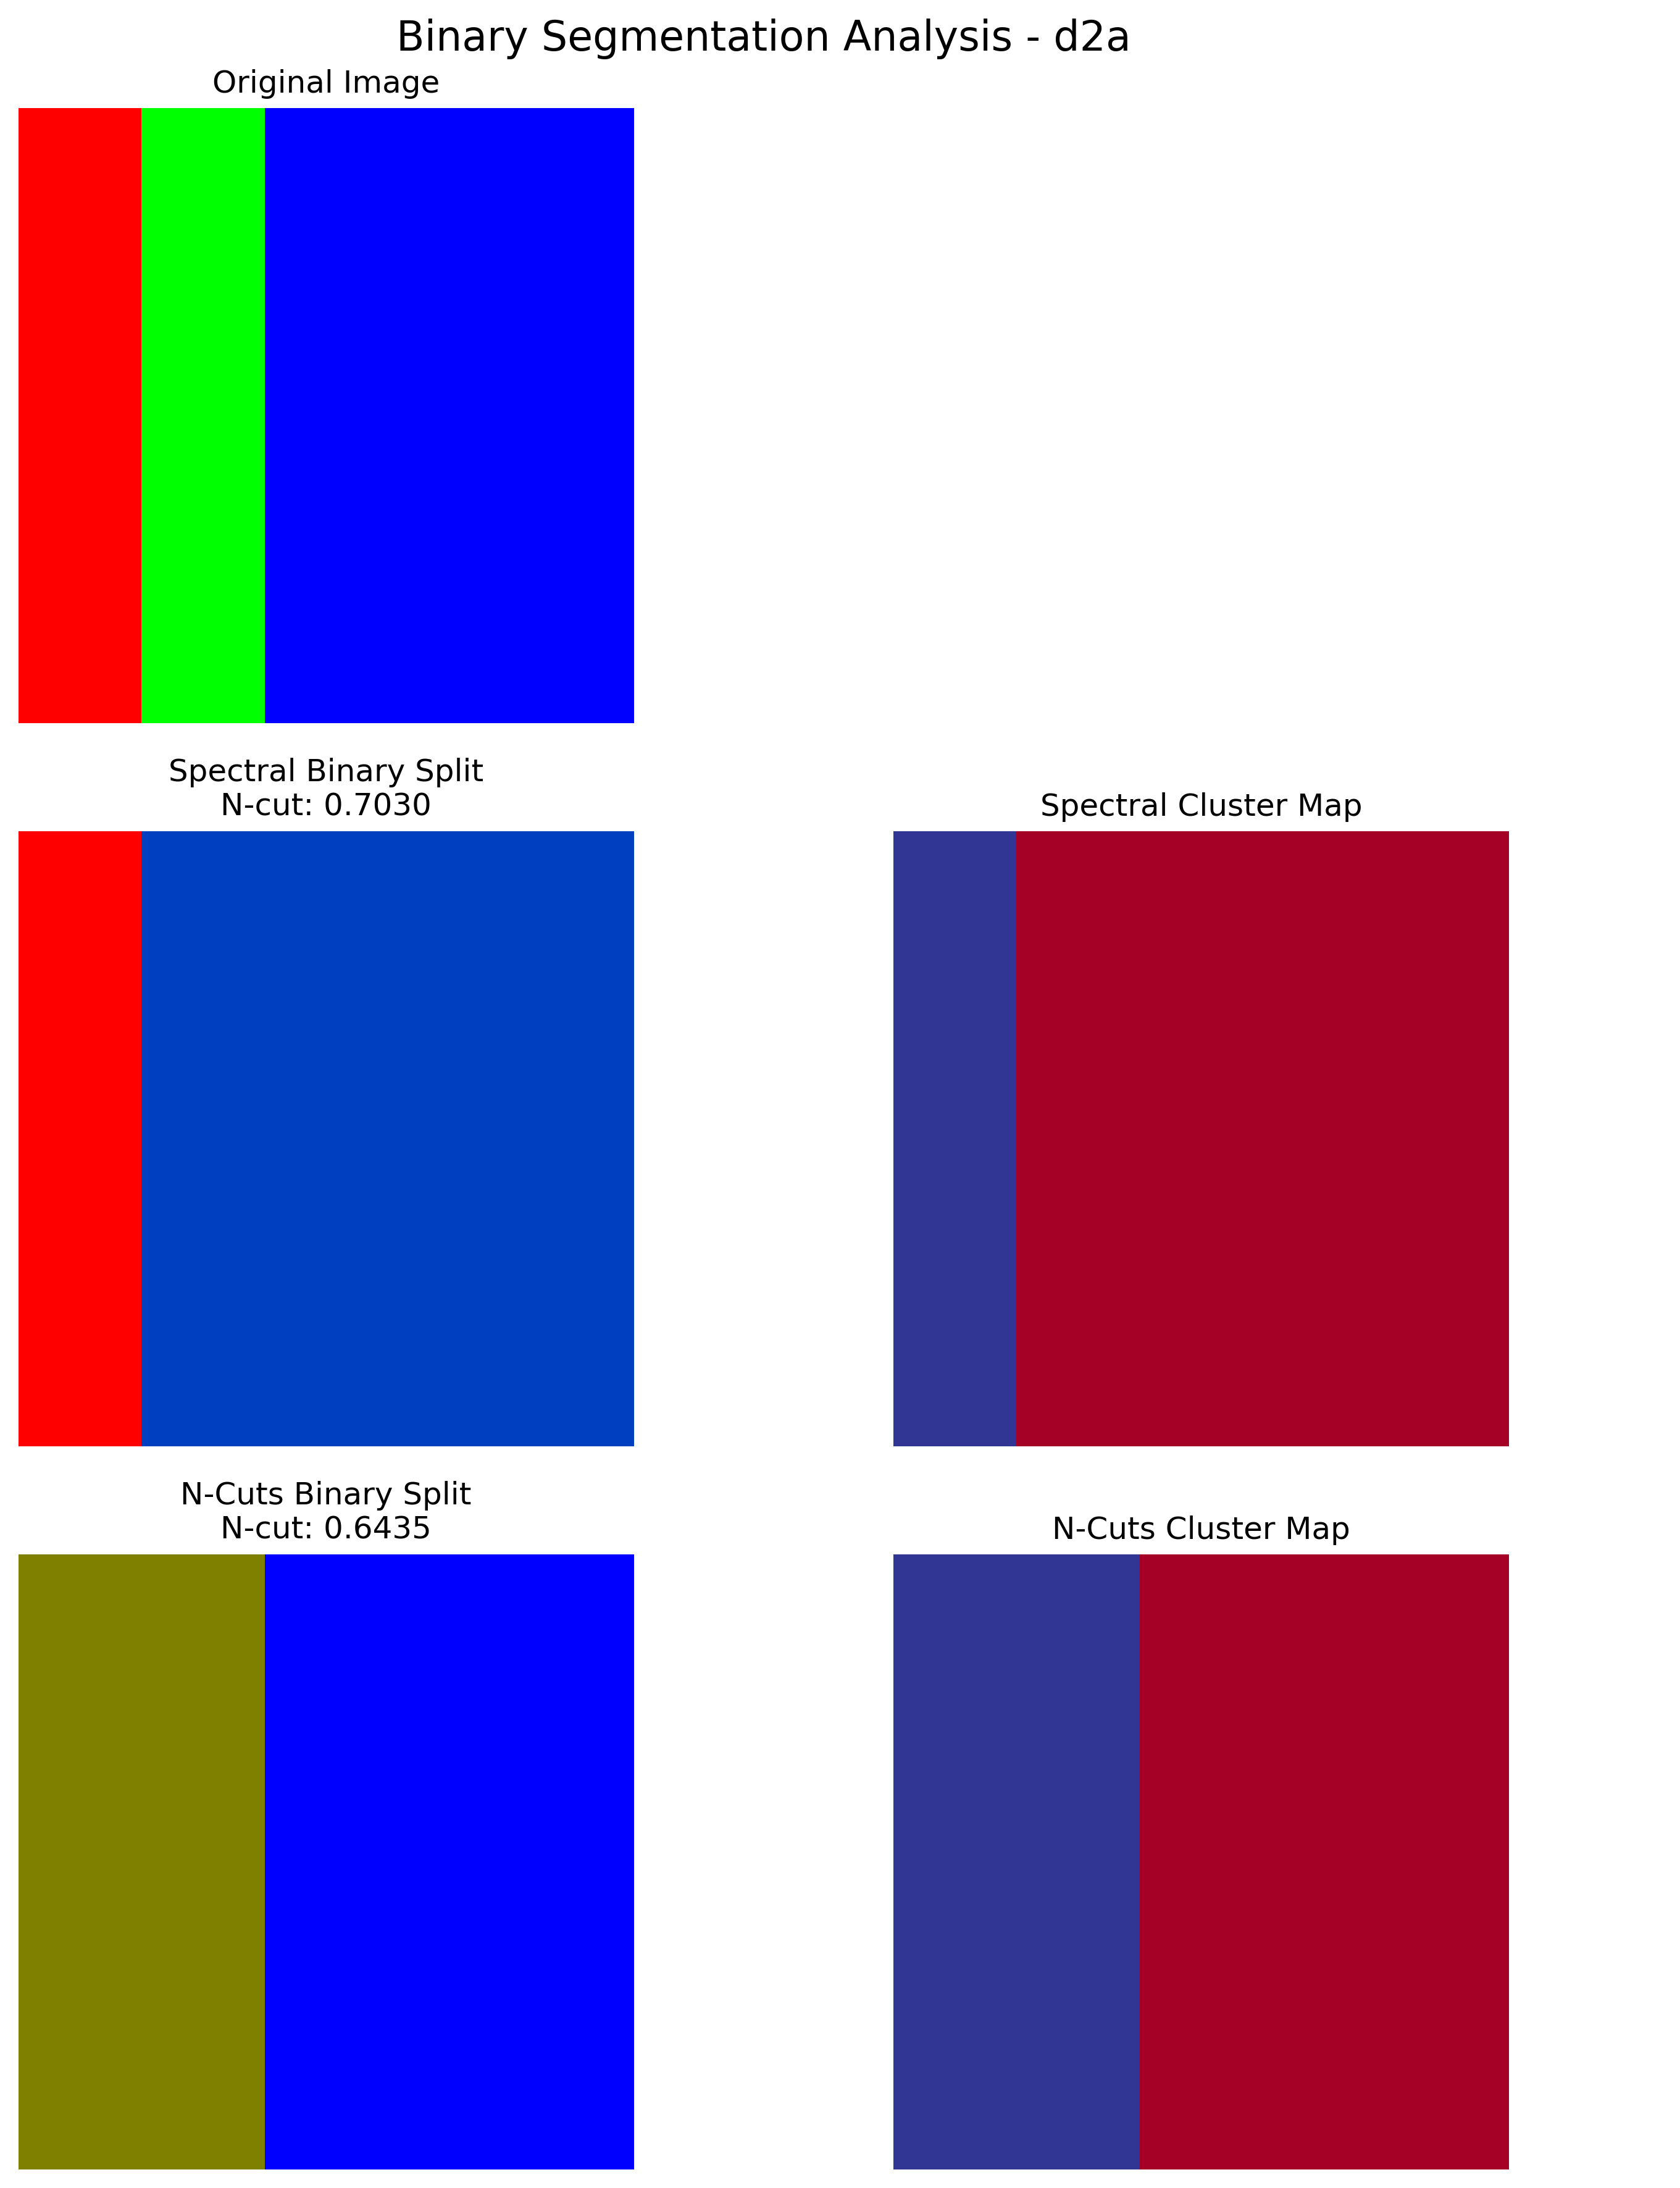
\includegraphics[width=\textwidth]{input/d2a.png}
        \caption{Image d2a (Three-stripe pattern)}
        \label{fig:d2a_original}
    \end{subfigure}
    \hfill
    \begin{subfigure}{0.45\textwidth}
        \centering
        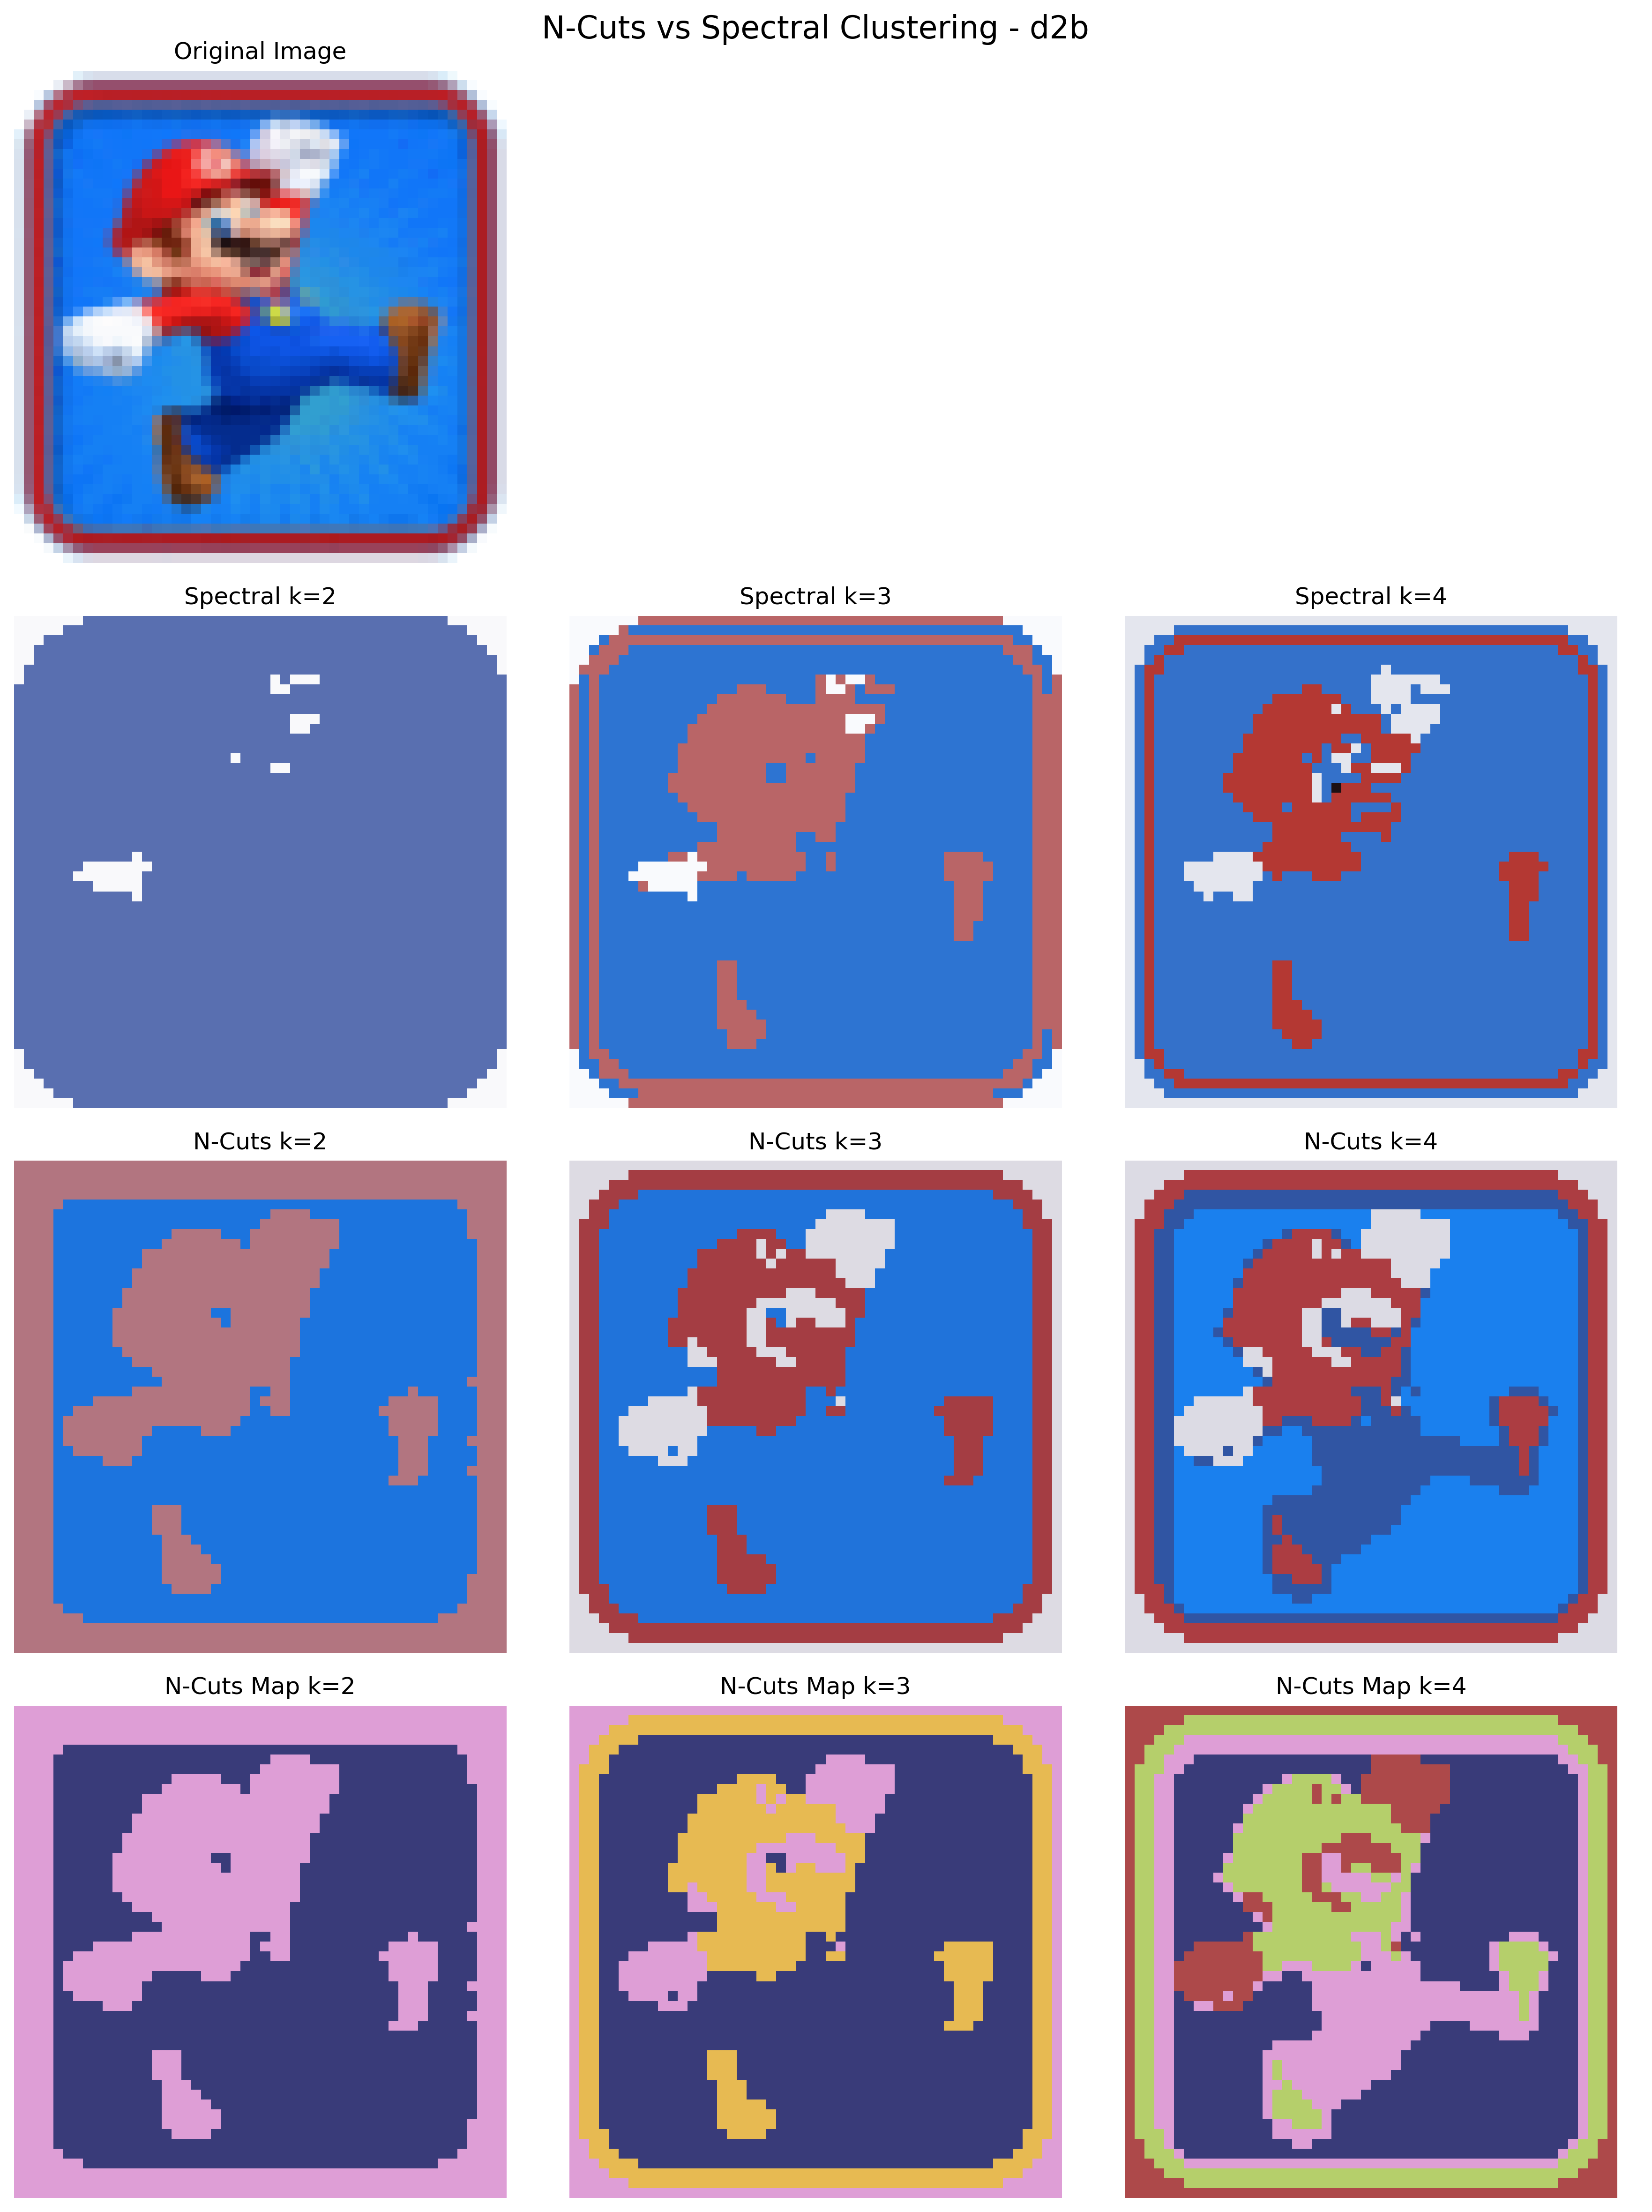
\includegraphics[width=\textwidth]{input/d2b.png}
        \caption{Image d2b (Mario character)}
        \label{fig:d2b_original}
    \end{subfigure}
    \caption{Test images used in the segmentation experiments}
    \label{fig:test_images}
\end{figure}








\section{Affinity Matrix Analysis}

The affinity matrix structure provides fundamental insights into the graph representation of images and reveals how pixel relationships are encoded for subsequent spectral clustering operations. This section presents a detailed analysis of affinity matrices for two distinct image types: a structured three-stripe pattern and a complex natural image.

\subsection{Simple Structured Image: Three-Stripe Pattern Analysis}


\subsubsection{Overall Matrix Structure}

The affinity matrix for the three-stripe test image (Figure~\ref{fig:affinity_matrix}) exhibits a characteristic \textbf{block diagonal structure} that directly mirrors the spatial organization of the input image. This structure manifests as:

\begin{itemize}
    \item \textbf{High-affinity blocks} (bright yellow regions, $W_{ij} = 1.0$): Represent strong intra-cluster connections between pixels within the same color region
    \item \textbf{Low-affinity blocks} (dark purple regions, $W_{ij} \approx 0$): Represent weak inter-cluster connections between pixels from different color regions
\end{itemize}


\begin{figure}[H]
    \centering
    \includegraphics[width=\textwidth]{demo2_affinity/demo2_affinity_d2a_results.png}
    \caption{Affinity matrix visualization for the three-stripe test image}
    \label{fig:affinity_matrix}
\end{figure}



\subsubsection{Detailed Block Analysis}

The matrix structure can be systematically analyzed through its constituent blocks, as highlighted in the red square region of Figure~\ref{fig:affinity_matrix} (the remaining areas show repetitions of this fundamental pattern):

\begin{enumerate}
    \item \textbf{Red Stripe Block (Upper-left)}: Corresponds to the first $n_r$ rows and columns, where $n_r$ is the number of red pixels. This block exhibits maximum internal affinity due to the uniform red coloration.
    
    \item \textbf{Green Stripe Block (Middle)}: Occupies the central portion of the matrix with dimensions $n_g \times n_g$. Similar to the red block, it shows high internal connectivity.
    
    \item \textbf{Blue Stripe Block (Lower-right)}: Forms the largest block due to the blue stripe occupying the majority of the image area. This creates a prominent high-affinity square in the bottom-right corner.
\end{enumerate}

\paragraph{Cross-Block Relationships:} The off-diagonal blocks reveal inter-stripe relationships. Due to the use of distinct RGB colors in the three-stripe pattern, all cross-block transitions exhibit uniformly low affinity values. This sharp and uniform transition between high intra-cluster affinity ($W_{ij} = 1.0$) and low inter-cluster affinity ($W_{ij} \approx 0$) creates an ideal structure for spectral clustering algorithms.



\subsection{Complex Natural Image: Mario Character Analysis}

The Mario character image (Figure~\ref{fig:affinity_matrix_mario}) presents a fundamentally different and more complex affinity matrix structure, characterized by:

\begin{itemize}
    \item \textbf{Mosaic Block Pattern}: The matrix is composed of multiple distinct blocks of varying sizes. As seen in the zoomed-in view, these blocks correspond to different color regions in the image (e.g., red for the hat, blue for overalls, distinct skin tones, and the background).
    \item \textbf{Graduated Affinity Values}: Unlike the simple binary affinity of the striped pattern, this matrix displays a continuous spectrum of intermediate values (green and teal colors, approx. 0.6-0.8). These values indicate partial similarities between related but not identical colors (e.g., different shades of red or blue).
    \item \textbf{Hierarchical Organization}: The presence of both large, dominant blocks (like the background) and smaller, nested blocks suggests a natural hierarchy. This structure implies that the image can be segmented at different levels of granularity, from broad regions down to fine details.
\end{itemize}


\begin{figure}[H]
    \centering
    \includegraphics[width=\textwidth]{demo2_affinity/demo2_affinity_d2b_results.png}
    \caption{Affinity matrix visualization for the Mario character image}
    \label{fig:affinity_matrix_mario}
\end{figure}



\newpage


\section{Demonstrations and Results}
The following subsections detail the five demonstration scripts and their outcomes.

\subsection{Demo 1: Spectral Clustering on Pre-built Affinity Matrix}
\textbf{Purpose}: Validate \texttt{spectral\_clustering} implementation on the provided affinity matrix.

\begin{figure}[H]
    \centering
    \includegraphics[width=0.3\textwidth]{input/d1a2.png}
    \caption{Input affinity matrix d1a}
    \label{fig:demo1}
\end{figure}

\textbf{Analysis}: The affinity matrix \texttt{d1a} is designed with three distinct high-affinity blocks along its diagonal, indicating a graph with three natural clusters. The connections within these blocks are strong, while inter-cluster affinities are low.
\begin{itemize}
    \item \textbf{For k=2 (Under-segmentation)}: The algorithm is forced to partition the data into fewer clusters than naturally exist. As a result, it merges two of the three distinct clusters into a single group, failing to capture the true underlying structure.
    \item \textbf{For k=3 (Correct Segmentation)}: When $k$ is set to 3, the algorithm perfectly identifies the three natural clusters defined by the high-affinity blocks in the matrix. This result validates that the implementation correctly finds the optimal partitioning when the number of clusters matches the data's structure.
    \item \textbf{For k=4 (Over-segmentation)}: The algorithm is forced to find more clusters than are naturally present. It correctly identifies the three main groups but then proceeds to split one of them into two smaller sub-clusters.
\end{itemize}
This demonstration confirms that the spectral clustering implementation works as expected, and highlights the critical importance of selecting the correct number of clusters, $k$.


\begin{figure}[H]
    \centering
    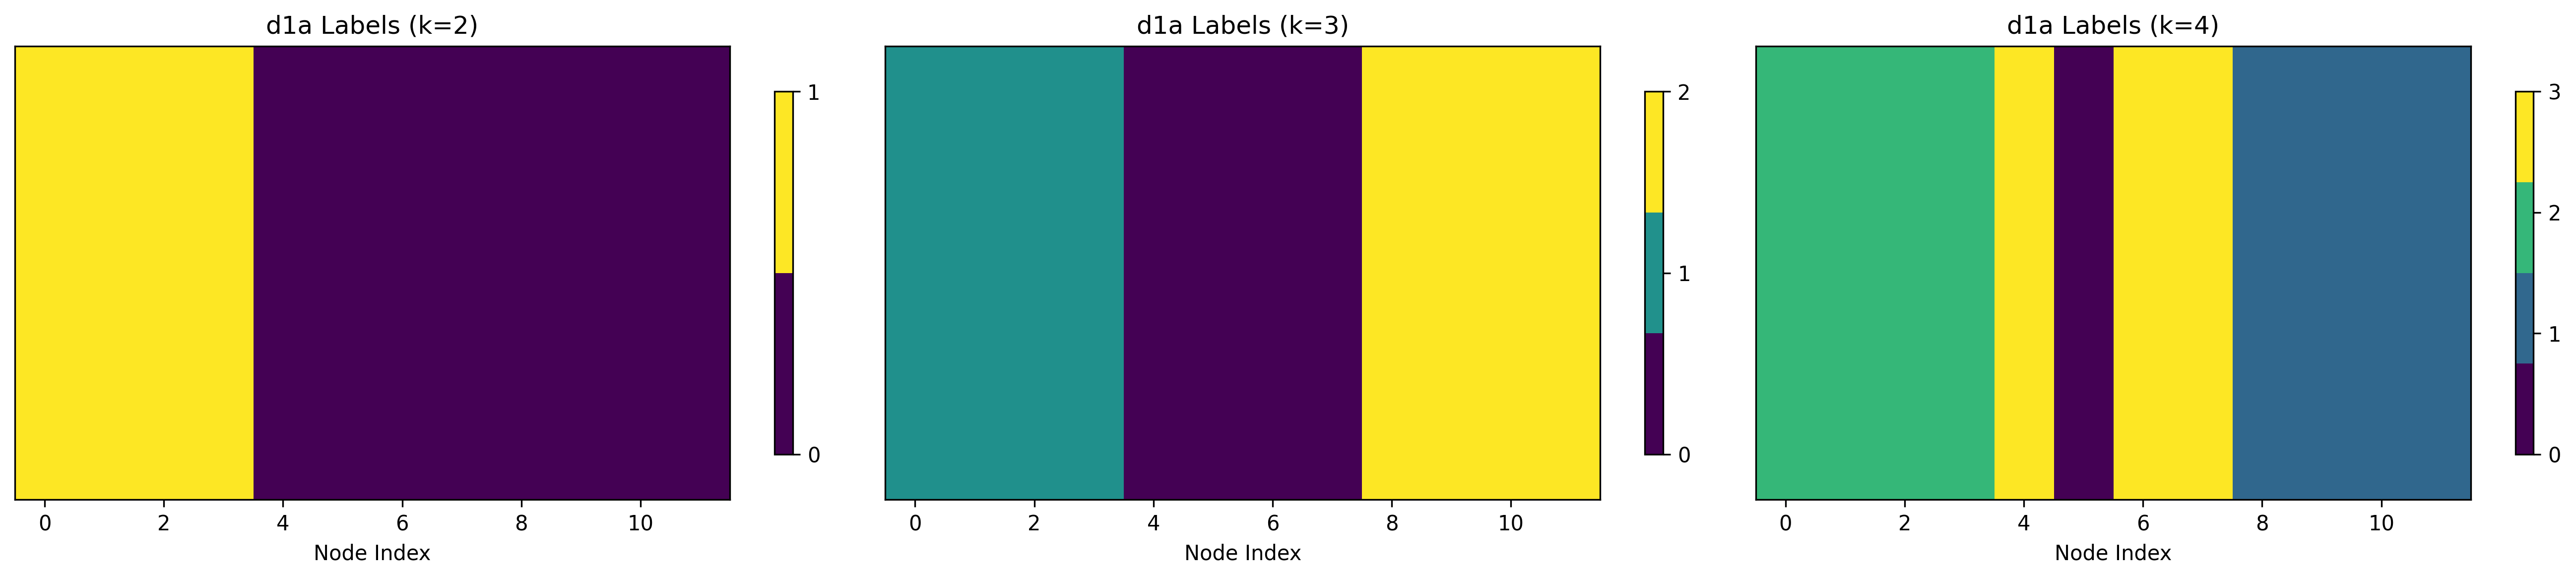
\includegraphics[width=\textwidth]{images/demo1_results.png}
    \caption{Spectral clustering results on pre-built affinity matrix d1a.}
    \label{fig:demo1}
\end{figure}


\subsection{Demo 2: Complete Pipeline (Image-to-Graph + Spectral Clustering)}
\textbf{Purpose}: To demonstrate the full workflow from raw image to segmentation using \texttt{image\_to\_graph} followed by \texttt{spectral\_clustering}. Tested on images \texttt{d2a} and \texttt{d2b}.

\subsubsection{Analysis of Image \texttt{d2a}}
The simple three-stripe image provides a clear test of the algorithm's ability to handle well-defined regions. The results demonstrate the critical impact of the parameter $k$:

\begin{figure}[H]
    \centering
    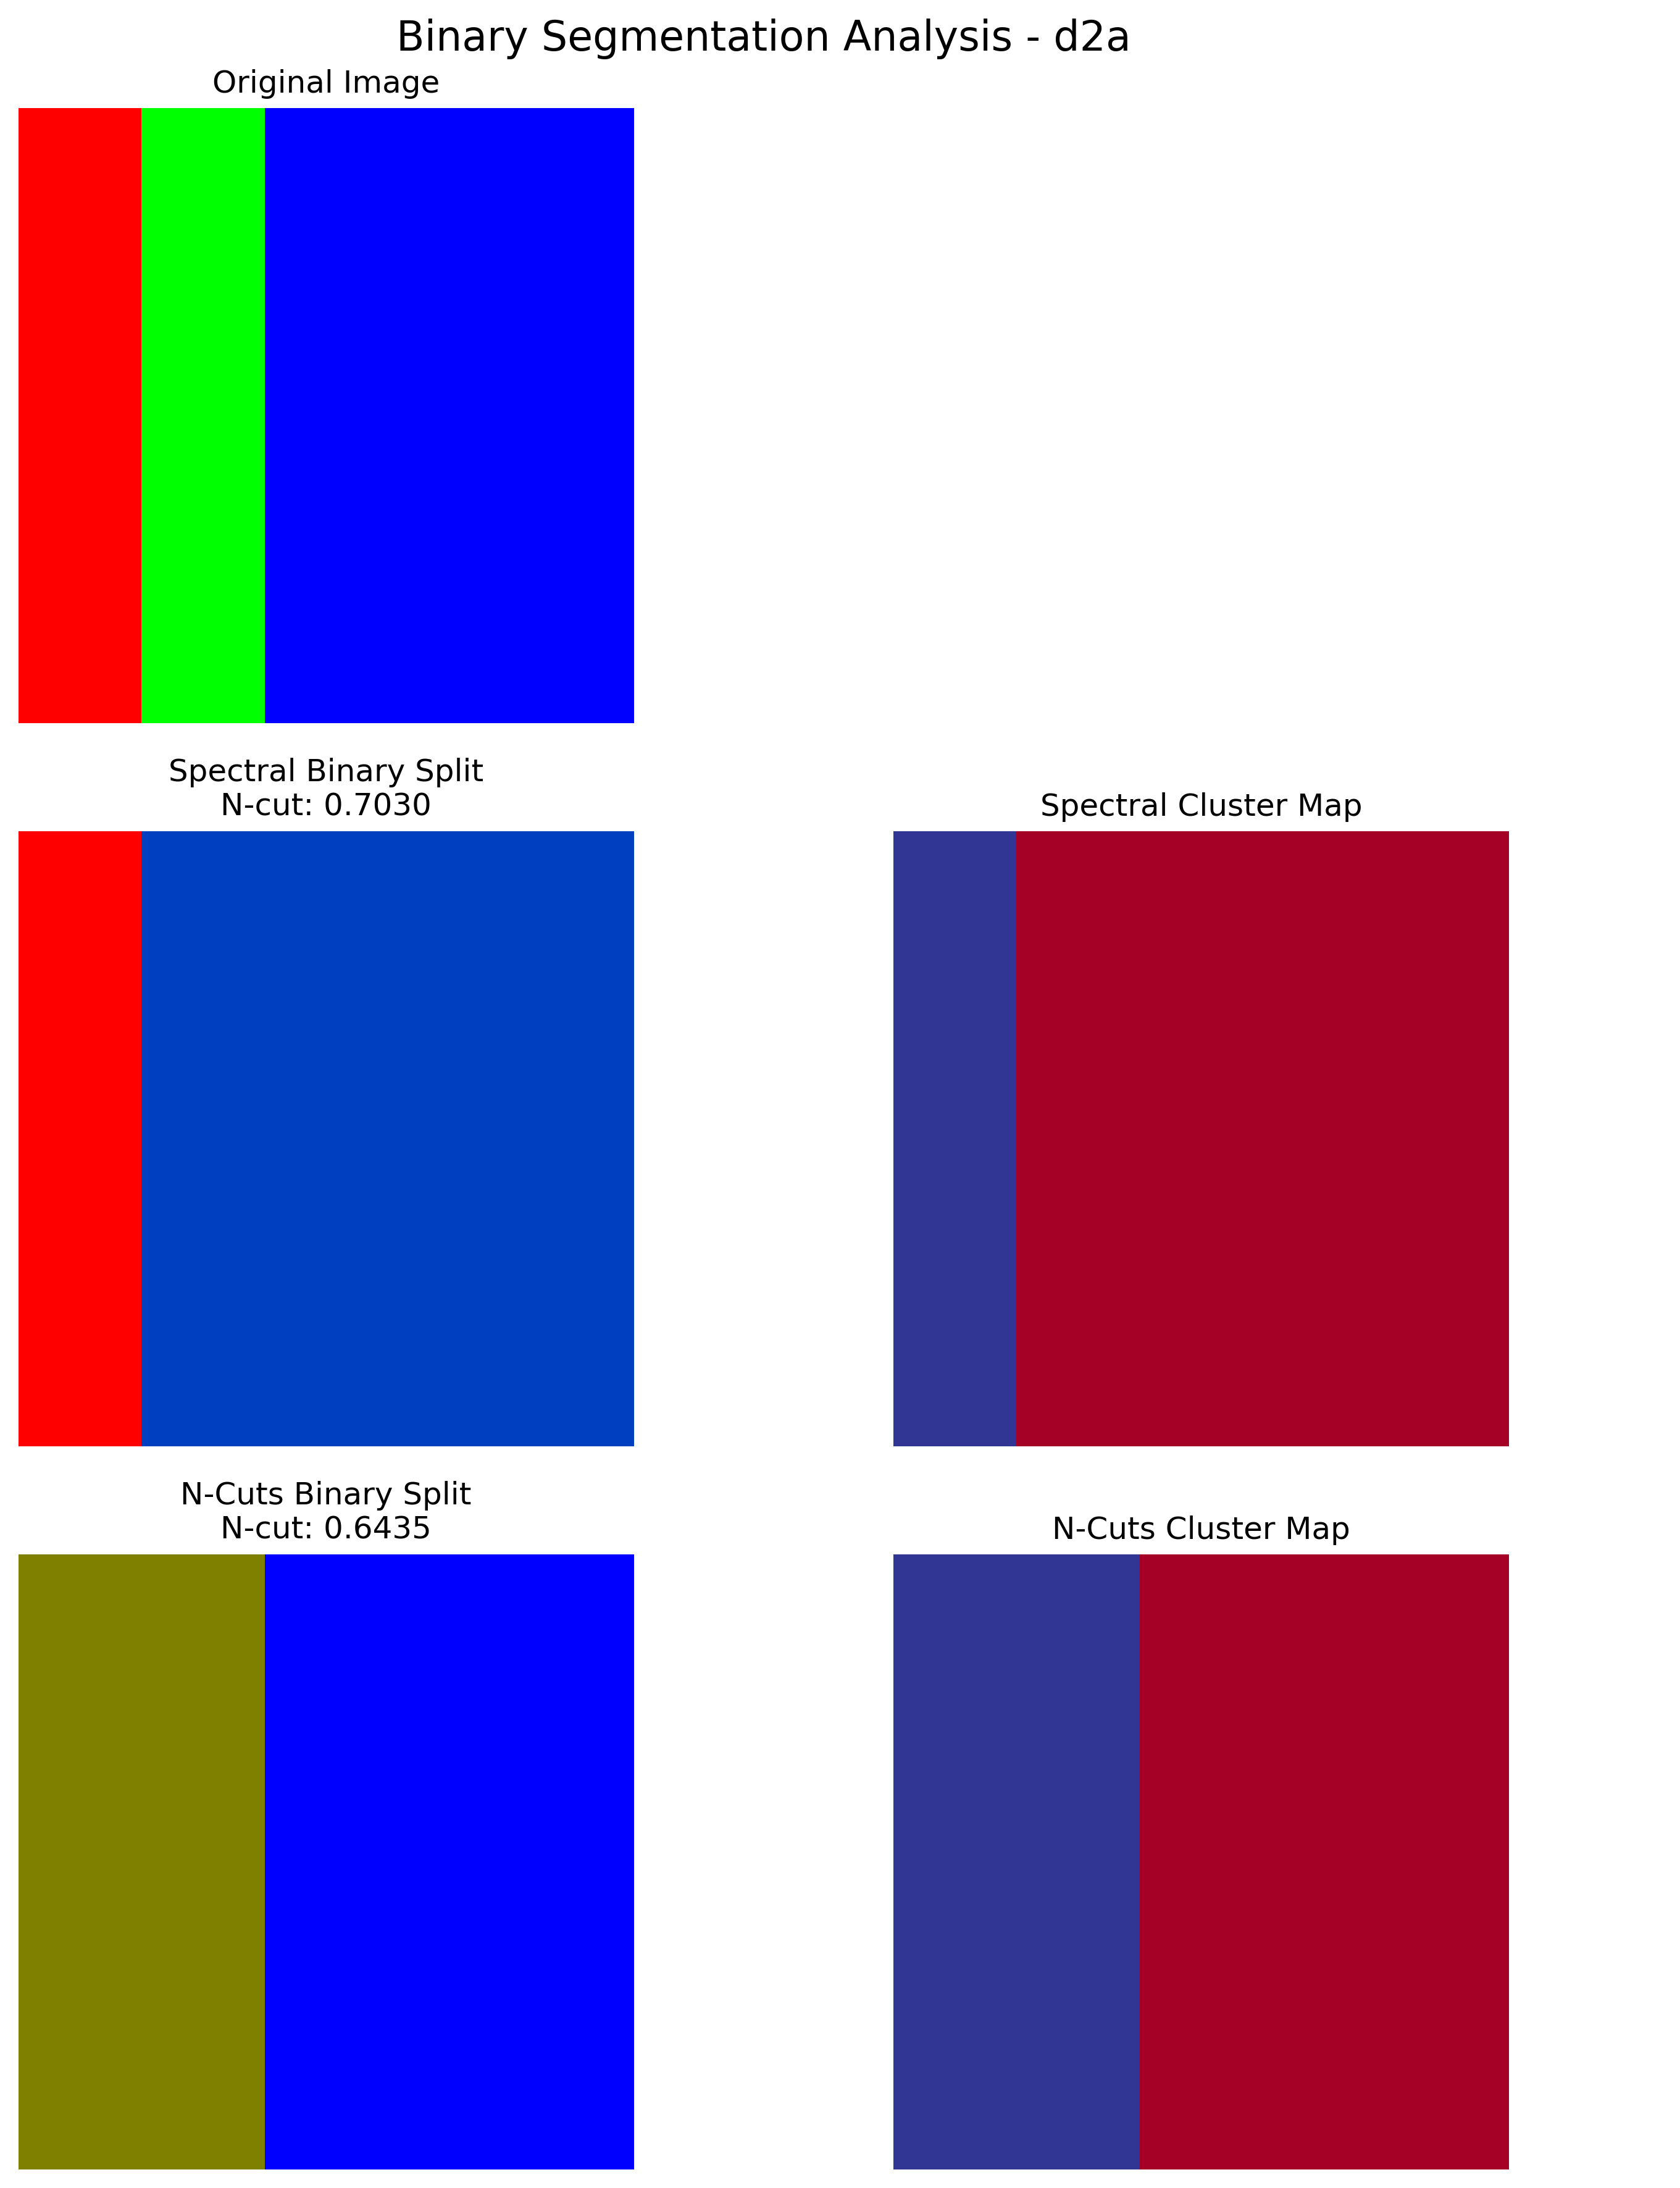
\includegraphics[width=0.5\textwidth]{input/d2a.png}
    \caption{Input image d2a}
    \label{fig:input_d2a}
\end{figure}

\begin{itemize}
    \item \textbf{For k=2 (Under-segmentation)}: The algorithm correctly identifies one of the primary color boundaries, separating the red stripe into its own cluster. However, being forced to create only two partitions, it groups the remaining green and blue stripes together into a single cluster.
    \item \textbf{For k=3 (Correct Segmentation)}: With $k$ set to the ground-truth number of regions, the algorithm performs perfectly. It accurately identifies and separates the red, green, and blue stripes into three distinct clusters, validating the pipeline's effectiveness when the correct number of clusters is known.
    \item \textbf{For k=4 (Over-segmentation)}: The algorithm is forced to find more clusters than naturally exist. Given that the image contains only three distinct colors, the algorithm correctly identifies the three main stripes but then incorrectly partitions some pixels into a fourth group without a clear criterion, leading to a flawed segmentation.
\end{itemize}

\begin{figure}[H]
    \centering
    \includegraphics[width=\textwidth]{images/demo2_d2a_results.png}
    \caption{Demo 2: Spectral Clustering on image \texttt{d2a} for $k=2,3,4$}
    \label{fig:demo2_d2a_results}
\end{figure}

\subsubsection{Analysis of Image \texttt{d2b}}
The Mario image presents a more complex challenge with multiple color regions of varying sizes.

\begin{figure}[H]
    \centering
    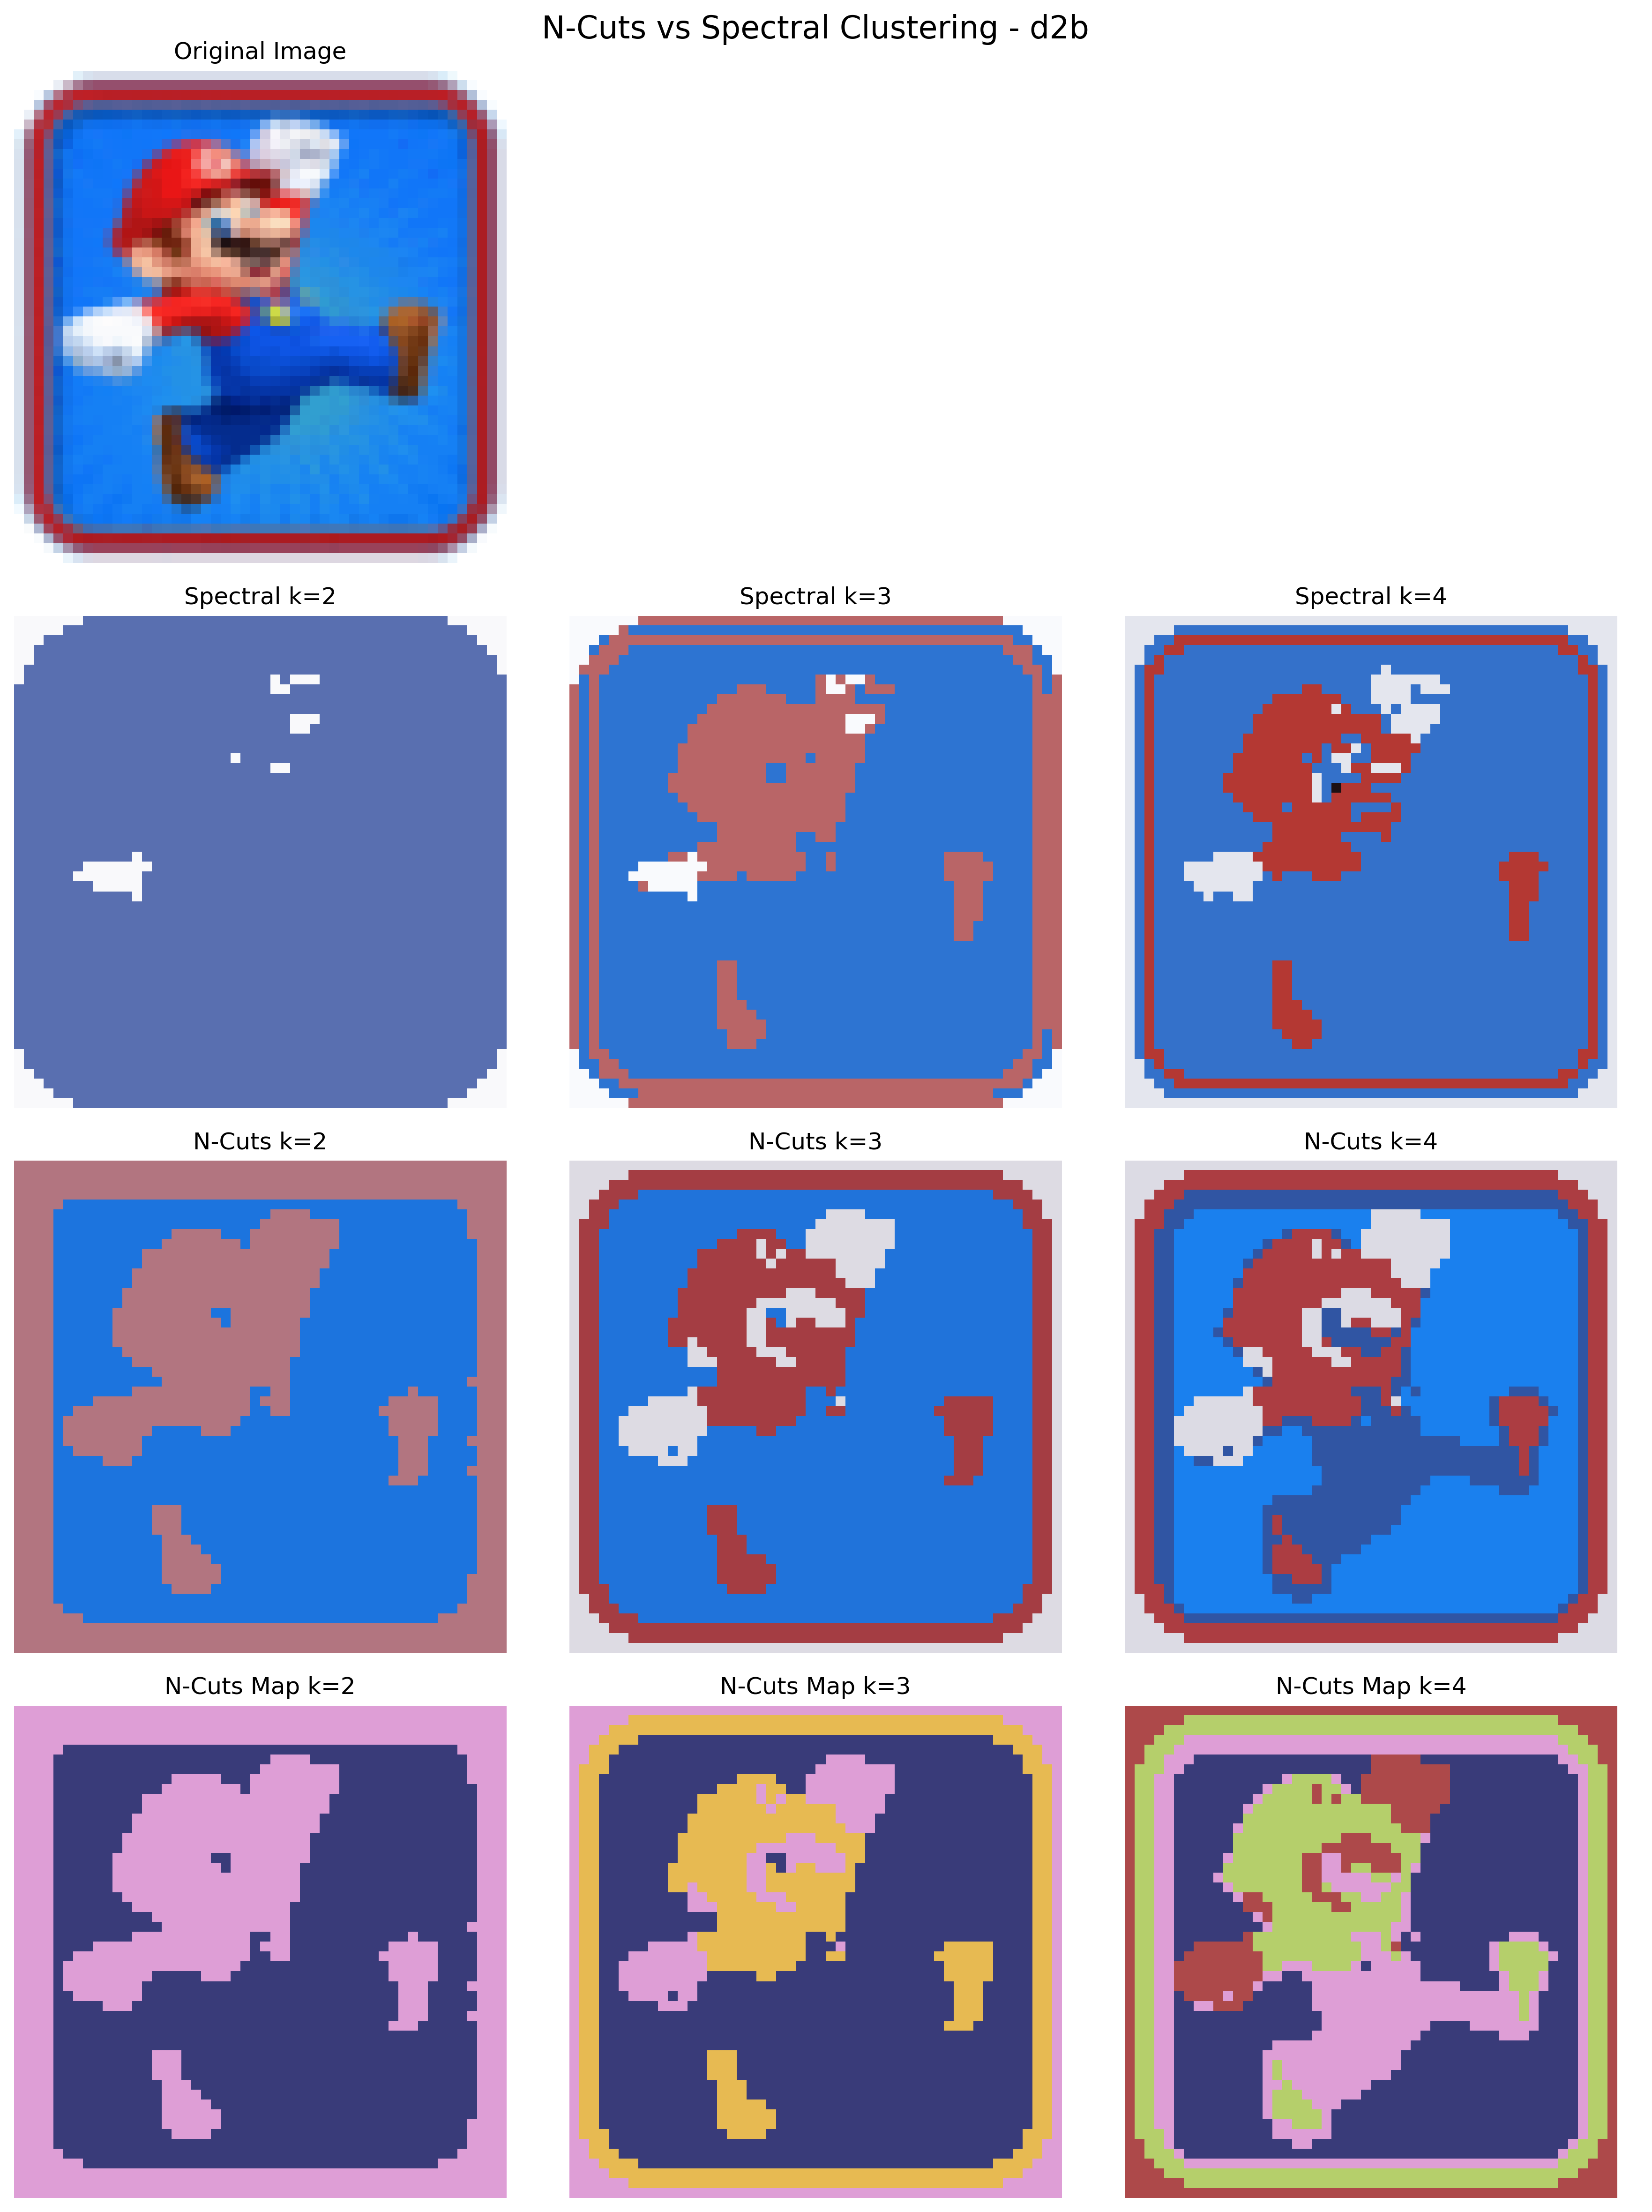
\includegraphics[width=0.5\textwidth]{input/d2b.png}
    \caption{Input image d2b}
    \label{fig:input_d2b}
\end{figure}

\begin{itemize}
    \item \textbf{For k=2}: The algorithm performs a basic binary split. A rough separation between the white parts of the character (gloves) and the blue background is visible, though the overall segmentation is very coarse.
    \item \textbf{For k=3}: The segmentation improves significantly. We can distinguish three clear groups: (1) the red features (hat, shirt, shoes), (2) the white features (gloves), and (3) the blue background.
    \item \textbf{For k=4}: Increasing the number of clusters to four does not yield any noticeable improvement in the segmentation quality compared to the k=3 result. 
\end{itemize}

\begin{figure}[H]
    \centering
    \includegraphics[width=\textwidth]{images/demo2_d2b_results.png}
    \caption{Demo 2: Spectral Clustering on image \texttt{d2b} for $k=2,3,4$}
    \label{fig:demo2_d2b_results}
\end{figure}



\subsection{Demo 3a: Non-Recursive N-Cuts vs Spectral Clustering}
\textbf{Purpose}: Compare non-recursive N-Cuts with spectral clustering on images \texttt{d2a} and \texttt{d2b}. This highlights differences arising from the standard vs. normalized Laplacian approaches.

\subsubsection{Analysis of Image \texttt{d2a}}

For the simple three-stripe image, both methods perform similarly, as the clusters are well-defined.

\begin{figure}[H]
    \centering
    \includegraphics[width=\textwidth]{images/demo3a_d2a_results.png}
    \caption{Demo 3a: N-Cuts vs Spectral Clustering on \texttt{d2a} for $k=2,3,4$}
    \label{fig:demo3a_d2a_results}
\end{figure}

\begin{itemize}

    \item \textbf{For k=2}: Both methods correctly identify one of the primary color boundaries. However, N-Cuts produces a more balanced partition by grouping the two smaller stripes (red and green) against the largest one (blue), whereas spectral clustering isolates the smallest stripe (red) from the other two. This highlights the balancing property of N-Cuts.
    \item \textbf{For k=3}: Both algorithms perform perfectly, correctly identifying the three distinct color stripes. With a clear ground truth, the normalization in N-Cuts does not provide a significant advantage over the standard approach.
    \item \textbf{For k=4}: Both methods are forced to over-segment the three natural stripes, but they handle this constraint differently. Spectral clustering distributes the over-segmentation across multiple stripes, creating additional partitions in both the red and green regions. In contrast, N-Cuts demonstrates more conservative behavior by maintaining the integrity of the smaller stripes (red and green) and only subdividing the largest region (blue stripe). This results in N-Cuts creating a fourth cluster with just 3 pixels from the blue stripe, while preserving the natural boundaries of the red and green stripes. This behavior illustrates N-Cuts' preference for balanced partitioning—it targets the largest cluster for subdivision rather than arbitrarily fragmenting smaller, well-defined regions.
\end{itemize}


\subsubsection{Analysis of Image \texttt{d2b}}

On the more complex Mario image, the differences between the two methods become more apparent, especially in how they handle regions of varying sizes.


\begin{figure}[H]
    \centering
    \includegraphics[width=\textwidth]{images/demo3a_d2b_results.png}
    \caption{Demo 3a: N-Cuts vs Spectral Clustering on \texttt{d2b} for $k=2,3,4$}
    \label{fig:demo3a_d2b_results}
\end{figure}


\begin{itemize}

    \item \textbf{For k=2}: N-Cuts demonstrates its superior performance by producing a more balanced and meaningful binary partition. It successfully separates the main character (grouping the red, white, and skin tones) from the blue background. In contrast, standard spectral clustering isolates the smallest, most distinct color group—the white gloves—from the rest of the image, demonstrating its tendency to create unbalanced cuts.

    \item \textbf{For k=3}: Both methods identify the main color groups (red features, blue background, and white elements), but N-Cuts demonstrates superior spatial coherence. The normalized cut criterion helps maintain connected regions, whereas spectral clustering produces a result with less coherent boundaries, exhibiting more noise and fragmentation, particularly in the character's features.
    
    \item \textbf{For k=4}: N-Cuts provides a more refined segmentation, beginning to separate the character's body/skin from the background, creating a fourth meaningful cluster. Spectral clustering fails to produce a useful fourth cluster, instead fragmenting existing regions without adding semantic value. 
\end{itemize}

\textbf{Comparative Summary}: N-Cuts consistently outperforms standard Spectral Clustering in producing more balanced, spatially coherent, and perceptually meaningful segmentations, particularly evident in complex images with multiple regions of varying sizes.


\subsection{Demo 3b: Quantitative Analysis of Binary Partitioning}
\textbf{Purpose}: To quantitatively evaluate the quality of a single binary partition ($k=2$) generated by both N-Cuts and standard spectral clustering.

This demonstration performs a single binary split on images \texttt{d2a} and \texttt{d2b}. Since this is equivalent to the non-recursive algorithms with a fixed $k=2$, the resulting segmented images are identical to those presented in Demo 3a (Figures \ref{fig:demo3a_d2a_results} and \ref{fig:demo3a_d2b_results}). The primary focus here is not on the visual output, but on the quantitative comparison of the partition quality using the N-Cut value as a metric. A lower N-Cut value is better.

\textbf{N-Cut Value Analysis:}
The table below presents the calculated N-Cut values for the binary partitions produced by each method. The results confirm that the N-Cuts algorithm achieves a more favorable (lower) N-Cut value for both images, validating its theoretical advantage in finding balanced cuts.

\begin{table}[H]
\centering
\begin{tabular}{@{}lcccc@{}}
\toprule
Image & N-Cuts Value & Spectral Value & Improvement \\
\midrule
d2a & 0.509 & 0.571 & 10.9\% \\
d2b & 0.780 & 0.934 & 16.6\% \\
\bottomrule
\end{tabular}
\caption{N-cut values for binary partitioning (lower is better)}
\label{tab:demo3b}
\end{table}

For the simple \texttt{d2a} image, N-Cuts provides an 10.9\% better N-Cut score. The improvement is even more pronounced on the complex \texttt{d2b} image, where N-Cuts achieves a 16.6\% lower N-Cut value. This quantitatively demonstrates that the normalization in the N-Cuts formulation leads to a superior partitioning solution compared to the unnormalized spectral clustering approach, especially for complex images.




\subsection{Demo 3c: Complete Recursive N-Cuts}
\textbf{Purpose}: To run the complete \texttt{n\_cuts\_recursive} algorithm with different threshold configurations on \texttt{d2a} and \texttt{d2b}. This demonstrates adaptive segmentation where the number of clusters is determined by the algorithm, and compares the impact of threshold selection on segmentation granularity.


\subsubsection{Threshold Analysis and Stopping Behavior}

The recursive N-Cuts algorithm begins with an initial binary split and evaluates whether to continue subdividing based on the quality thresholds. From Demo 3b, we obtained the following quantitative results for the initial binary partitions:

\begin{table}[H]
\centering
\begin{tabular}{@{}lcc@{}}
\toprule
Image & N-Cut Value & Cluster Sizes \\
\midrule
d2a & 0.509 & [1500, 1000] \\
d2b & 0.780 & [1361, 1139] \\
\bottomrule
\end{tabular}
\caption{Initial binary split results for recursive N-Cuts}
\label{tab:demo3c_initial}
\end{table}

\subsubsection{Conservative Threshold Configuration ($T_1=5$, $T_2=0.20$)}

\textbf{Stopping Criterion Analysis}:
\begin{itemize}
    \item \textbf{For image d2a}: The initial binary split produces an N-Cut value of 0.509, which exceeds the threshold $T_2 = 0.20$. According to the recursive algorithm's stopping criteria, this split quality is insufficient to warrant further subdivision. The algorithm therefore terminates after the initial binary partition, resulting in exactly 2 final clusters.
    
    \item \textbf{For image d2b}: Similarly, the initial binary split yields an N-Cut value of 0.780, which significantly exceeds $T_2 = 0.20$. Consequently, the recursive algorithm stops after the initial split, producing 2 final clusters.
\end{itemize}

The choice of $T_2=0.20$ proves to be quite restrictive for both test images. This conservative threshold prevents further subdivision beyond the initial binary split, effectively making the recursive algorithm equivalent to a single binary N-Cuts operation.

\subsubsection{Permissive Threshold Configuration}

To demonstrate the adaptive nature of recursive N-Cuts and allow for more granular segmentation, we tested with relaxed thresholds tailored to each image's characteristics:

\begin{itemize}
    \item \textbf{For image d2a}: $T_1=5$, $T_2=0.55$ (allowing splits with N-Cut values up to 0.55)
    \item \textbf{For image d2b}: $T_1=5$, $T_2=0.85$ (allowing splits with N-Cut values up to 0.85)
\end{itemize}

\begin{table}[H]
\centering
\begin{tabular}{@{}lccc@{}}
\toprule
Image & Threshold $T_2$ & Final Clusters & Segmentation Quality \\
\midrule
d2a & 0.20 & 2 & Conservative (under-segmented) \\
d2a & 0.55 & 6 & Over-segmentation \\
d2b & 0.20 & 2 & Conservative (under-segmented) \\
d2b & 0.85 & 6 & More granular segmentation \\
\bottomrule
\end{tabular}
\caption{Comparison of recursive N-Cuts results with different threshold configurations}
\label{tab:demo3c_comparison}
\end{table}

\textbf{Results with Permissive Thresholds}:

\begin{figure}[H]
    \centering
    \includegraphics[width=\textwidth]{images/demo3c_d2a_results.png}
    \caption{Recursive N-Cuts results for image d2a with permissive threshold}
    \label{fig:demo3c_d2a}
\end{figure}

\textbf{Image d2a with $T_2=0.55$}: The initial N-Cut of 0.509 is now below the threshold, so the split is accepted. The algorithm proceeds to recursively subdivide the resulting clusters. As shown in Figure~\ref{fig:demo3c_d2a}, the algorithm successfully identifies and separates the three primary color stripes (red, green, blue). However, with the permissive threshold, it continues subdividing beyond the natural structure, creating additional segments within each color region. This results in 6 final clusters, representing an over-segmentation where each original stripe is further partitioned. While this demonstrates the algorithm's ability to find finer-grained structures, it exceeds the optimal segmentation for this simple image.

\begin{figure}[H]
    \centering
    \includegraphics[width=\textwidth]{images/demo3c_d2b_results.png}
    \caption{Recursive N-Cuts results for image d2b with permissive threshold}
    \label{fig:demo3c_d2b}
\end{figure}

\begin{itemize}     
    \item \textbf{Image d2b with $T_2=0.85$}: The initial N-Cut of 0.780 is below the new threshold, allowing the algorithm to proceed beyond the basic binary split. As illustrated in Figure~\ref{fig:demo3c_d2b}, the recursive process produces a much more detailed segmentation with 6 final clusters. The algorithm successfully separates different components of the Mario character: the red elements (hat, shirt), white elements (gloves), blue background, and additional fine-grained regions within the character. This demonstrates the algorithm's capacity to discover meaningful hierarchical structures in complex images when provided with appropriate thresholds.
\end{itemize}



\subsubsection{Implications of Threshold Selection}

This comparison reveals the critical role of threshold selection in recursive N-Cuts:

\begin{itemize}
    \item \textbf{Quality vs. Granularity Trade-off}: Conservative thresholds (low $T_2$ values) prioritize partition quality over granularity, potentially leading to under-segmentation. Permissive thresholds allow for more detailed segmentation but may accept lower-quality splits.
        
    \item \textbf{Adaptive Segmentation Advantage}: Unlike fixed-$k$ methods that force a predetermined number of clusters, recursive N-Cuts adapts to both the data structure and the specified quality requirements. With appropriate thresholds, it can discover the natural segmentation hierarchy present in the data.    
\end{itemize}

This demonstrates that recursive N-Cuts provides a powerful framework for adaptive image segmentation, where the choice of thresholds allows users to control the trade-off between segmentation quality and detail level according to their specific application.






\section{Discussion}
This section synthesizes the findings from the demonstrations and addresses key aspects of the implemented segmentation methods.

\subsection{Impact of Parameter $k$}
The choice of $k$ (number of clusters) is critical for non-recursive methods.
\begin{itemize}
    \item \textbf{Under-segmentation}: If $k$ is too small relative to the number of perceptually distinct regions, multiple regions will be merged into single segments.
    \item \textbf{Over-segmentation}: If $k$ is too large, perceptually single regions might be unnecessarily split into multiple segments.
    \item Demo 2 clearly showed how increasing $k$ from 2 to 4 leads to finer partitions. The optimal $k$ depends on the image content and the desired level of detail in the segmentation.
\end{itemize}

\subsection{Computational Considerations}
\begin{itemize}
    \item \textbf{Affinity Matrix Construction}: For an $M \times N$ image, the affinity matrix is $(MN) \times (MN)$. For a $50 \times 50$ image (625 pixels), this is $2500 \times 2500$. For a $100 \times 100$ image (10,000 pixels), this is $10,000 \times 10,000$. Storing and processing this dense matrix is computationally intensive. The implemented \texttt{image\_to\_graph} uses vectorized operations for efficiency.
    \item \textbf{Eigen-decomposition}: Computing eigenvalues/vectors is the most expensive step in spectral clustering and N-Cuts. Using \texttt{scipy.sparse.linalg.eigsh} to find only the $k$ smallest eigenvalues/vectors is crucial for larger matrices. 
    \item \textbf{K-Means}: Clustering in the $k$-dimensional eigenspace is relatively fast as $k$ is usually small. 
\end{itemize}
For larger images (e.g., $100 \times 100$ or more), these methods become very demanding in terms of memory and CPU time if applied to the full pixel graph. In practice, for larger images, they are often applied to superpixels.




\subsection{Future Improvements}

\begin{itemize}
    \item Develop adaptive parameter selection for recursive stopping criteria
    \item Explore GPU acceleration for matrix operations
    \item Incorporate spatial constraints in affinity computation
\end{itemize}



\section{Conclusion}
This project successfully implemented and demonstrated image segmentation using spectral clustering and normalized cuts. The image-to-graph conversion laid the foundation by representing pixel relationships as an affinity matrix. Spectral clustering provided a baseline graph partitioning method, while N-Cuts offered a more sophisticated approach aiming for balanced segments. The non-recursive versions of both highlighted the impact of the chosen number of clusters, $k$. The recursive N-Cuts algorithm showcased an adaptive segmentation strategy, capable of determining the number of segments based on intrinsic data properties and defined quality thresholds.

The demonstrations confirmed theoretical expectations: N-Cuts generally produces more balanced partitions than spectral clustering, and recursive N-Cuts offers adaptability that fixed-$k$ methods lack. The choice of algorithm and parameters ($k, T_1, T_2$) significantly influences the segmentation outcome and should be tailored to the specific image characteristics and application goals.



\begin{thebibliography}{9}

\bibitem{shi2000normalized}
Shi, J., \& Malik, J. (2000). Normalized cuts and image segmentation. \textit{IEEE Transactions on Pattern Analysis and Machine Intelligence}, 22(8), 888-905.

\bibitem{von2007tutorial}
Von Luxburg, U. (2007). A tutorial on spectral clustering. \textit{Statistics and Computing}, 17(4), 395-416.

\end{thebibliography}


\end{document}